\setcounter{page}{1}
\pagenumbering{arabic}
\chapter{Inleiding}
\label{ch:Inleiding}
Menselijke actieherkenning is het proces dat op een automatische manier (I) detecteert dat een persoon een bepaalde actie uitvoert en (II) herkennen welke actie dit is. Voorbeelden van zulke acties zijn lopen, stappen, zwaaien, springen, bukken, enz. Actieherkenning kent tal van toepassingen, voornamelijk bij de interactie tussen mens en computer, zoals fysiotherapie \cite{Deboeverie2017}, lichaamsanalyse \cite{Devi2015} en 





\section{Probleemstelling}
Actieherkenning kan opgesplitst worden in twee onderdelen: actiedetectie en de actieherkenning zelf. Voor actieherkenning is er al uitbundig onderzoek gedaan naar allerlei verschillende manieren om effectief acties te herkennen. Vaak wordt er gebruik gemaakt van histogrammen \cite{Xia2012},
\cite{Chen2017},
\cite{Vezzani2010},
\cite{Mendoza2007}, \todo{andere vaak gebruikte dingen zoeken}


Actieherkenning en actiedetectie blijft moeilijk te realiseren in een real-time scenario, waarbij snelle beslissingen gemaakt moeten worden. Het doel van deze masterproef is om live classificatie van acties mogelijk te maken. 



\section{De Kinect}
De Kinect (figuur \ref{fig:KinectSensorVersies}) is origineel ontworpen als manier om de gebruiker zelf als spelcontroller te beschouwen. De Kinect bevat een kleurencamera, dieptesensor, \todo{eens experimenteren met kinect}. Door de goedkope technologie die de Kinect aanbiedt wordt de Kinect vaak gebruikt bij onderzoek in de computervisie. Voor actieherkenning kunnen zowel de kleurencamera als dieptesensor bijdragen tot actieherkenning. Enerzijds kunnen de kleurencamera en dieptesensor gecombineerd worden om RGB-D data te bekomen. Anderzijds kan vanuit het dieptebeeld een skelet gegenereerd worden via de methode van Shotton et al. \cite{Shotton2011}, die reeds ingebouwd zit in de Kinect.
\begin{figure}
	\begin{subfigure}[t]{0.48\textwidth}
		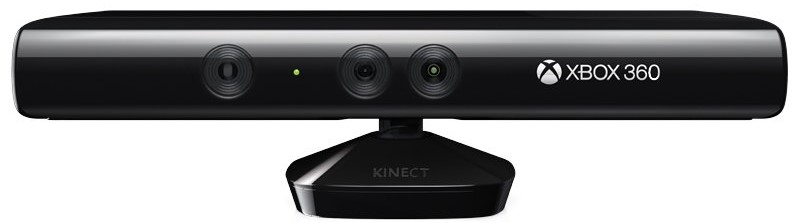
\includegraphics[width=\linewidth]{KinectSensor360}
		\caption{De originele Kinect sensor, ontwikkeld int 2010 voor de Xbox 360.}
	\end{subfigure}
	\begin{subfigure}[t]{0.48\textwidth}
		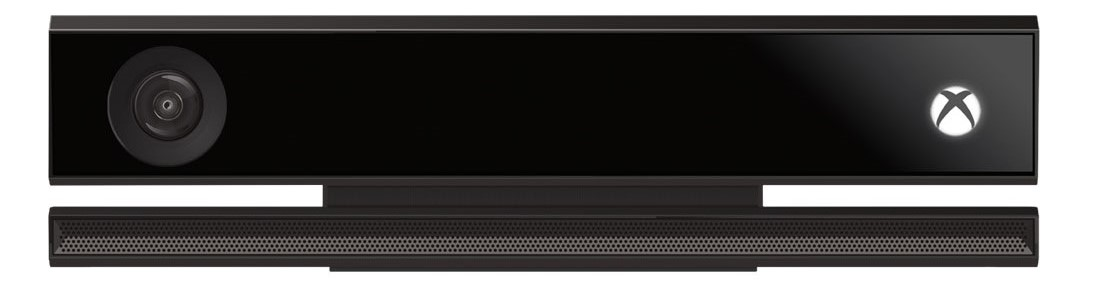
\includegraphics[width=\linewidth]{KinectSensorOne}
		\caption{De tweede iteratie van de Kinect sensor, specifiek gemaakt voor Xbox One en uitgebracht in 2013.}
		\label{fig:KinectSensorOne}
	\end{subfigure}
	\caption{Twee versies van de Kinect sensor.}
	\label{fig:KinectSensorVersies}
\end{figure}

Voor deze masterproef wordt de tweede versie van de Kinect gebruikt, die te zien is op figuur \ref{fig:KinectSensorOne}.


\section{Structuur}
Deze scriptie \todo{structuur, pas doen wanneer voldoende inhoud}
